% Chapter 4: Artificial Intelligence Features
\chapter{Artificial Intelligence Features}

\chapterquote{Artificial intelligence is the new electricity.}{Andrew Ng}

\section*{Introduction}
\addcontentsline{toc}{section}{Introduction}

This chapter explores the integration of artificial intelligence capabilities within our real estate platform. We have developed four distinct AI models, each addressing specific requirements within the ecosystem. These models collectively enhance user experience, improve decision-making processes, and provide valuable insights to various stakeholders in the real estate market.

The AI features presented in this chapter represent a significant competitive advantage for our platform, enabling more accurate property valuations, personalized recommendations, intelligent assistance, and efficient administrative operations. Each model has been carefully designed to solve real-world challenges faced by users interacting with real estate data and transactions.

\section{Sprint 2: Data Collection and Scraping}
\subsection*{Overview}
This section details the data collection processes implemented to gather the real estate market data required for our AI models. 

\subsection{Real Estate Data Scraping}
\subsubsection{Data Sources}
We identified several real estate websites with
significant listings for the Tunisian market: Properstar, Remax, Home in Tunisia, and
Mubawab. These platforms offered a reasonable volume of property listings with the
attributes needed for our models. For each website, I developed a dedicated Python
script that navigated through the listings, extracted the relevant property details, and
stored the information in CSV files. This approach gave us a foundation of raw data that
could later be processed and used for training our prediction models.
\newpage
\begin{figure}[htbp]
    \centering
    \begin{minipage}{0.47\textwidth}
        \centering
        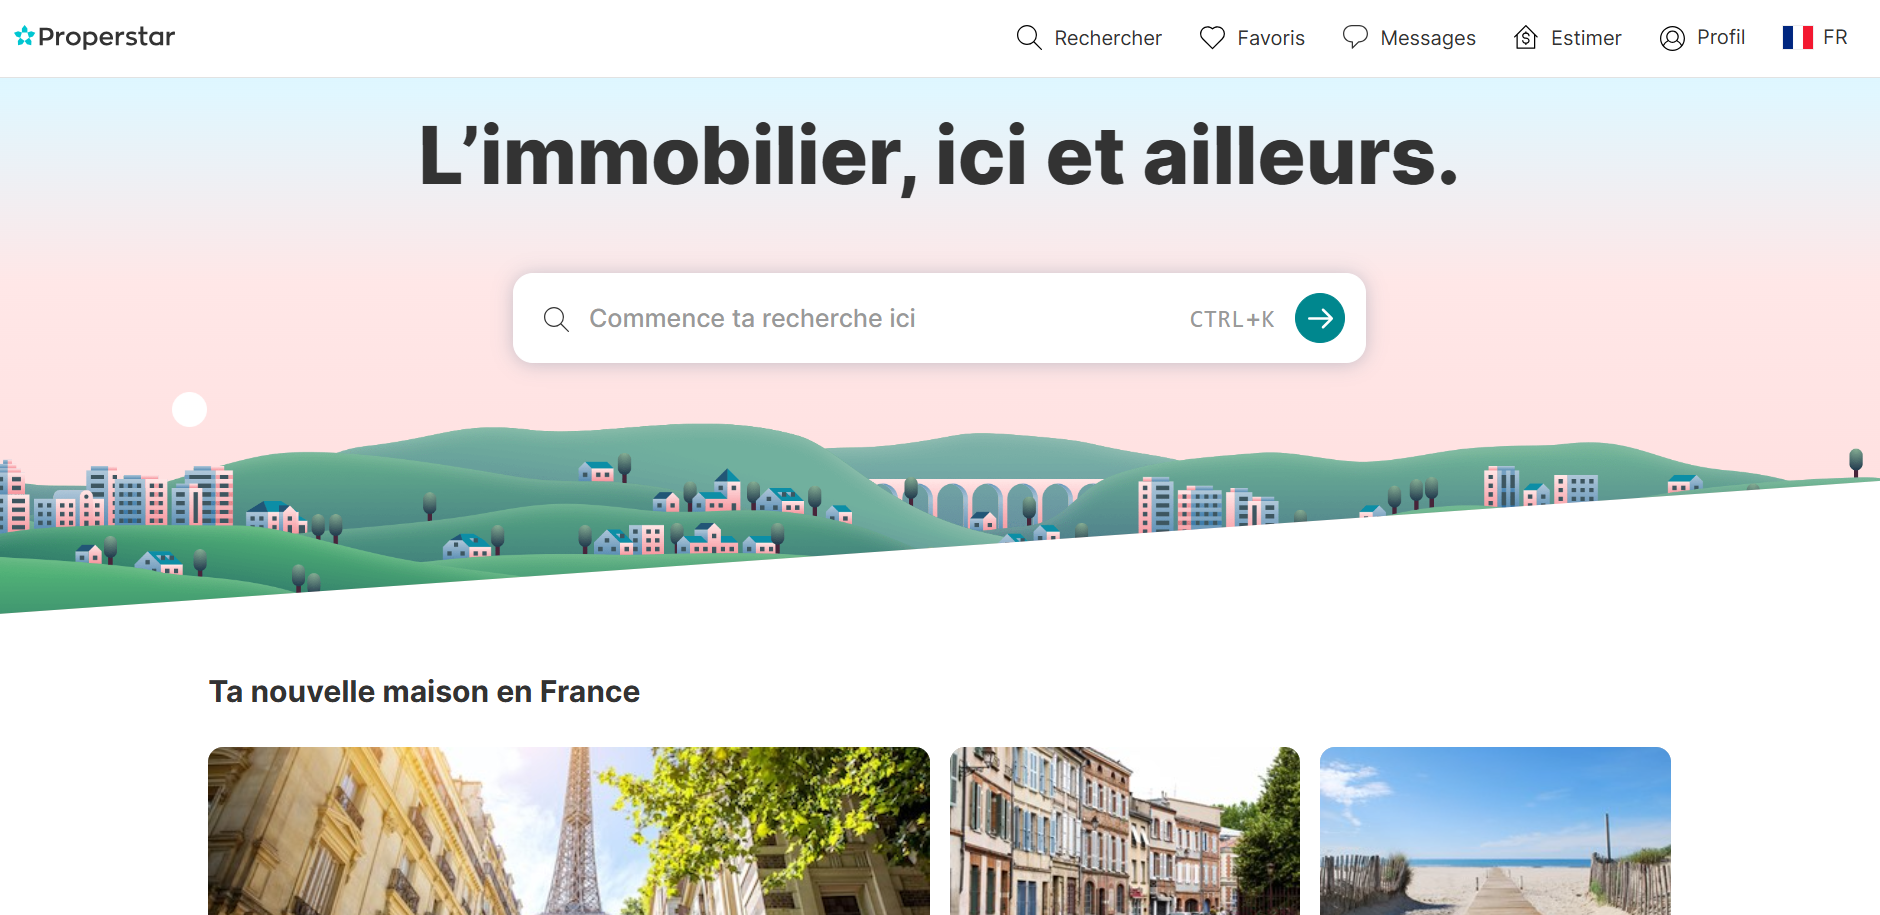
\includegraphics[width=\linewidth]{images/properstar.png}
        \caption{properstar website}
        \label{fig:properstar-website}
    \end{minipage}
    \hfill
    \begin{minipage}{0.47\textwidth}
        \centering
        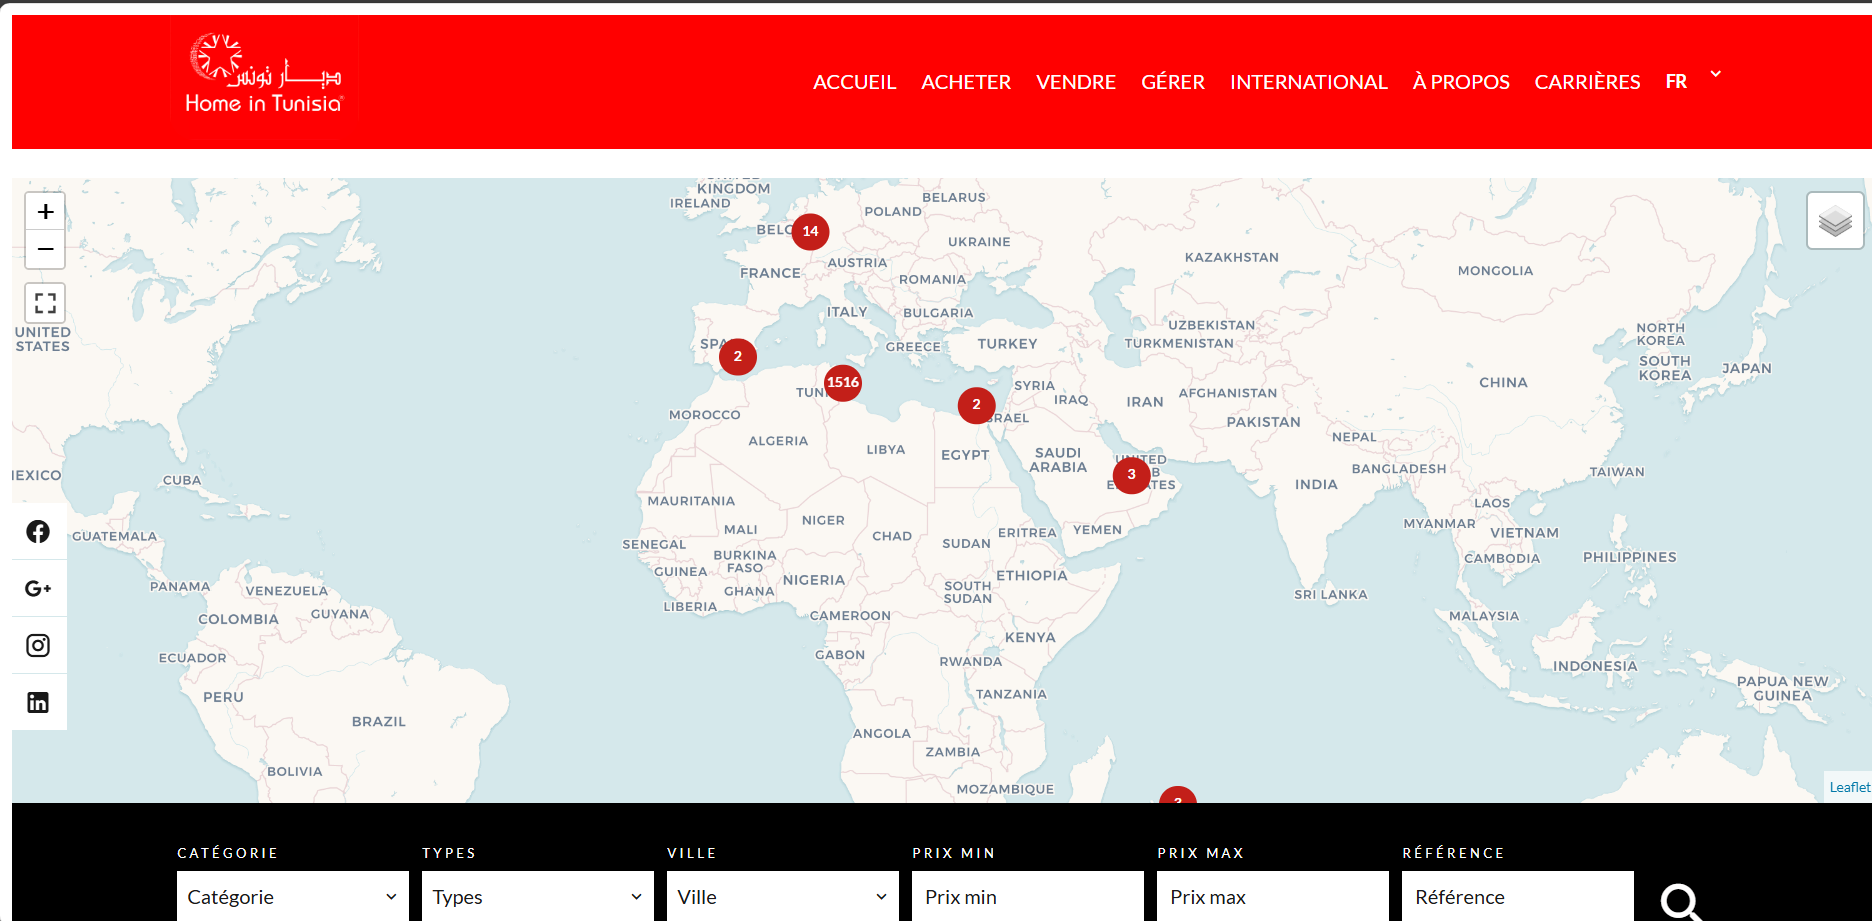
\includegraphics[width=\linewidth]{images/home_in_tunisia.png}
        \caption{homeintunisia website}
        \label{fig:homeintunisia-website}
    \end{minipage}
    
    \vspace{0.75cm}
    
    \begin{minipage}{0.47\textwidth}
        \centering
        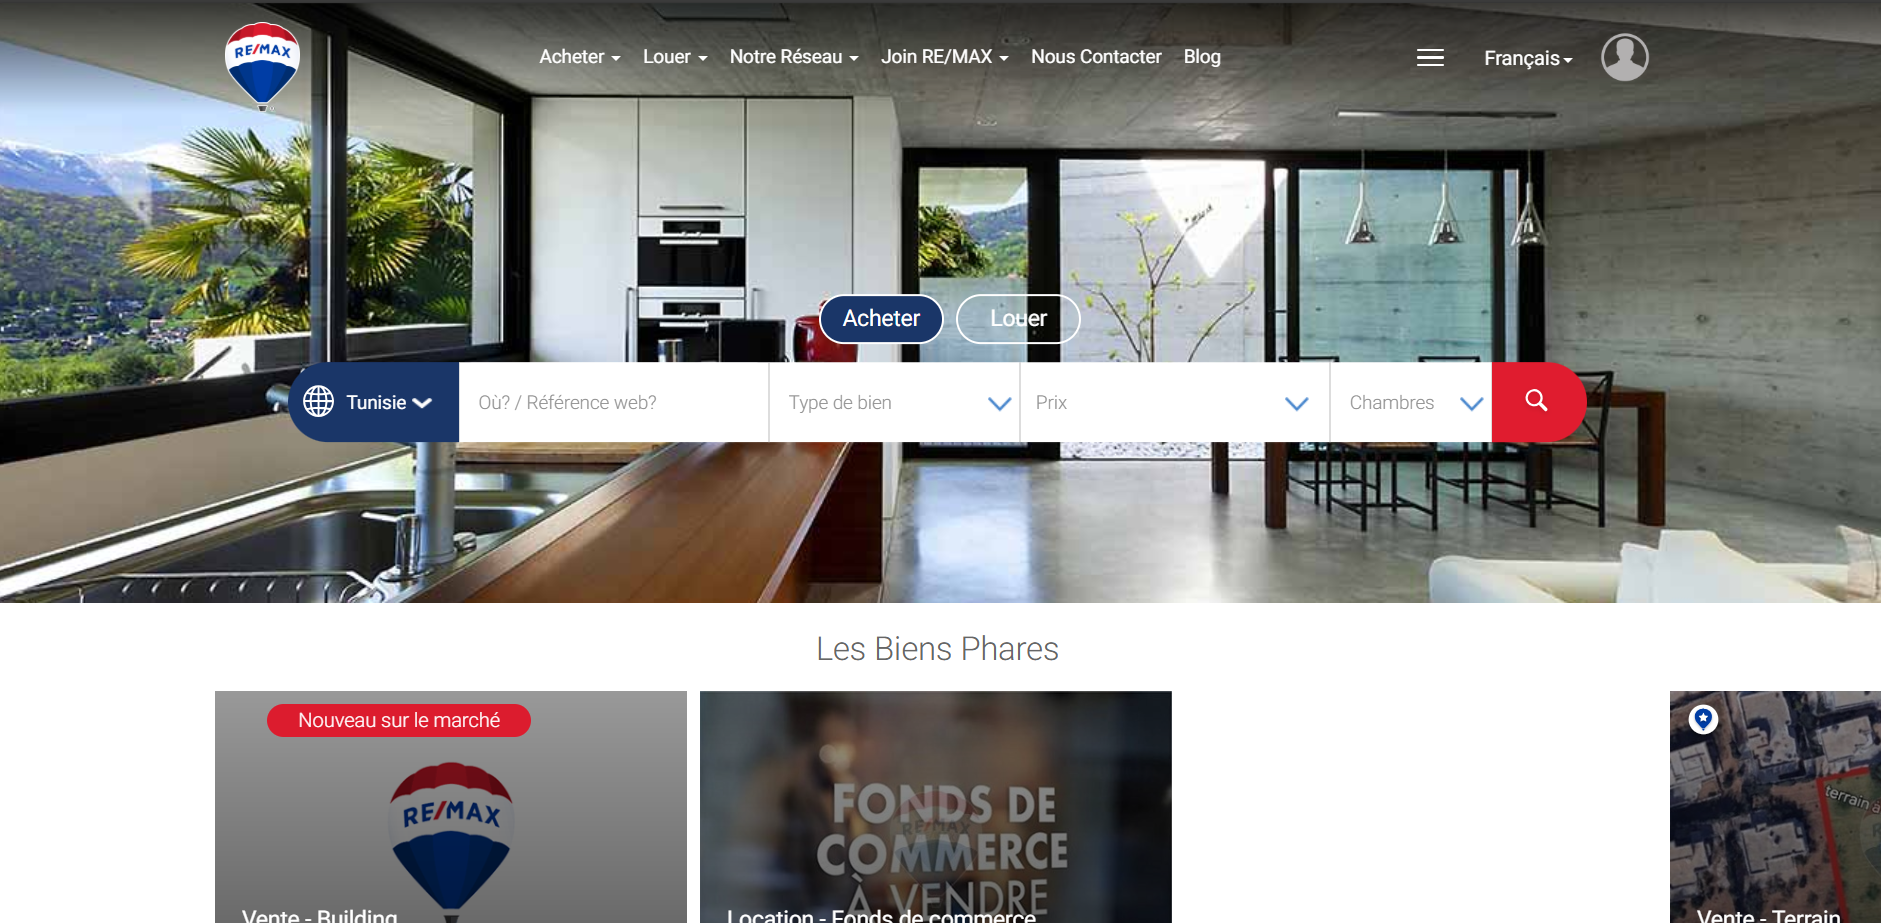
\includegraphics[width=\linewidth]{images/remax.png}
        \caption{remax website}
        \label{fig:remax-website}
    \end{minipage}
    \hfill
    \begin{minipage}{0.47\textwidth}
        \centering
        
\includegraphics[width=\linewidth]{images/mub.png}
        \caption{mubawab website}
        \label{fig:mubawab-website}
    \end{minipage}
\end{figure}

Our scraping system uses a distributed architecture with the following components:
\begin{itemize}
    \item Scheduled jobs for regular data updates, Data validation and cleaning pipelines
\end{itemize}

\begin{figure}[htbp]
    \centering
    % Placeholder for a diagram of the scraping workchart
    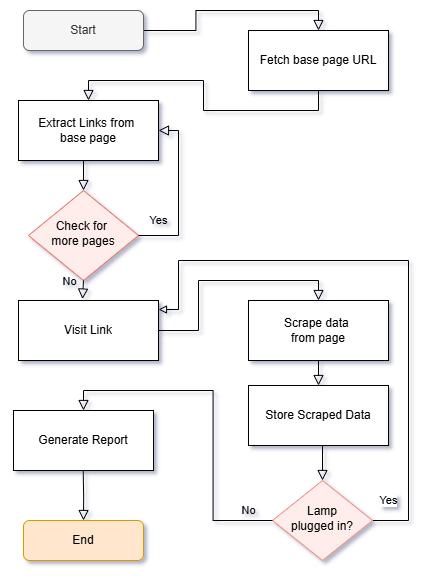
\includegraphics[width=0.35\textwidth]{images/workchartscraper.png}
    \caption{Data Scraping workchart}
    \label{fig:scraping-workchart}
\end{figure}

\section{Sprint 3: Property Valuation Prediction Model}
\subsection*{Overview}
The Property Valuation Prediction Model is designed to estimate both the market value and potential rental income for real estate properties. This provides investors with crucial information to make informed investment decisions.

\subsection{Requirements Analysis}
\subsubsection{Use Case Diagram}
The property valuation model serves multiple actors within the Korpor ecosystem. Figure \ref{fig:valuation-use-case} illustrates the primary use cases for the AI-powered property valuation system.

\begin{figure}[htbp]
    \centering
    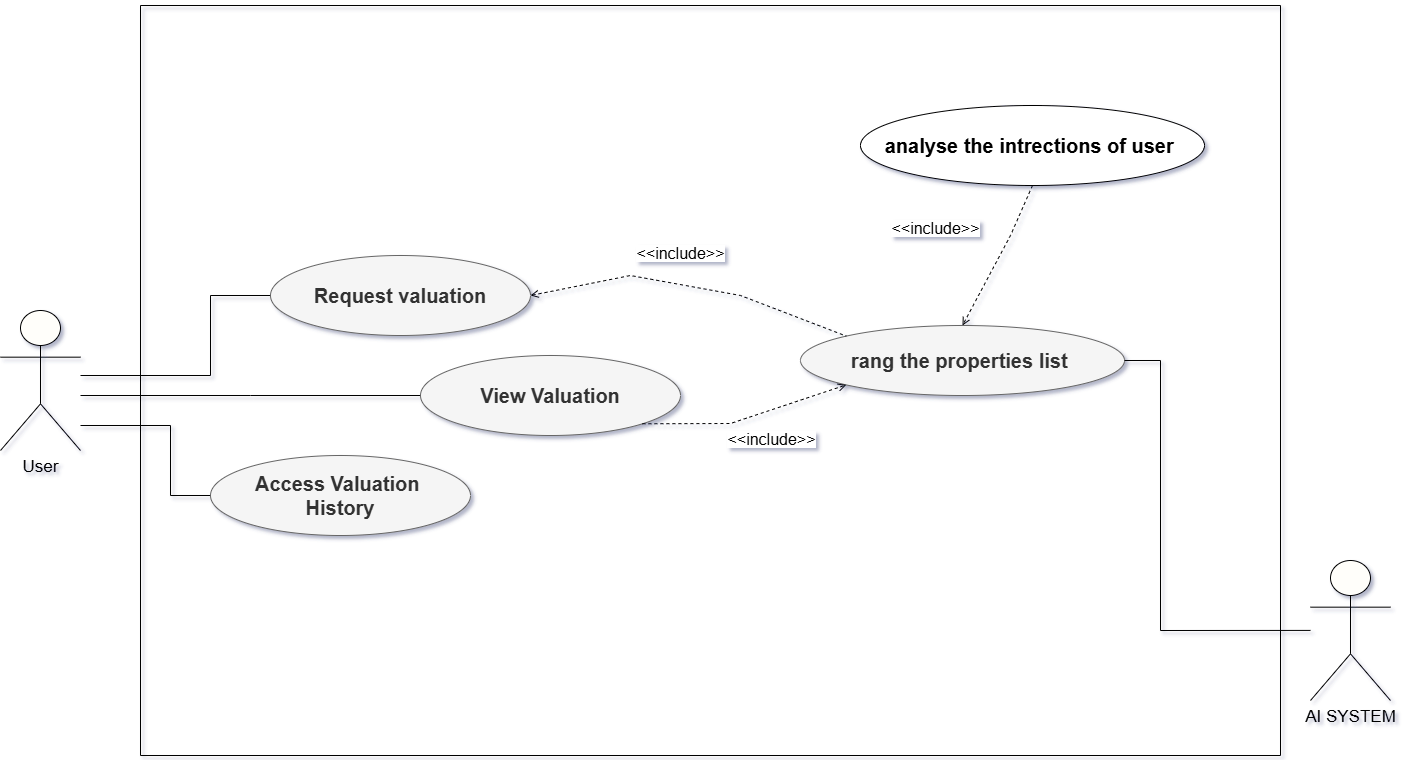
\includegraphics[width=0.8\textwidth]{images/valuation_use_case_diagram.png}
    \caption{Property Valuation Model Use Case Diagram}
    \label{fig:valuation-use-case}
\end{figure}

\subsubsection{Textual Use Case Descriptions}

\textbf{Use Case: Request Property Valuation}
\begin{itemize}
    \item \textbf{Actor}: User (representing Super Admin, Admin, Real Estate Agent)
    \item \textbf{Precondition}: User is authenticated and has access to valuation features
    \item \textbf{Main Flow}: 
    \begin{enumerate}
        \item User inputs property details (location, size, type, amenities)
        \item System validates input data
        \item System processes data through ML model
        \item System returns market value and rental income predictions
        \item User reviews and saves valuation results
    \end{enumerate}
    \item \textbf{Alternative Flow}: If data is incomplete, system requests additional information
    \item \textbf{Postcondition}: Valuation is stored and available for future reference
\end{itemize}

\subsection{System Design}
\subsubsection{Class Diagram}
The property valuation system follows object-oriented design principles. Figure \ref{fig:valuation-class-diagram} shows the main classes and their relationships.
\newpage

\begin{figure}[htbp]
    \centering
    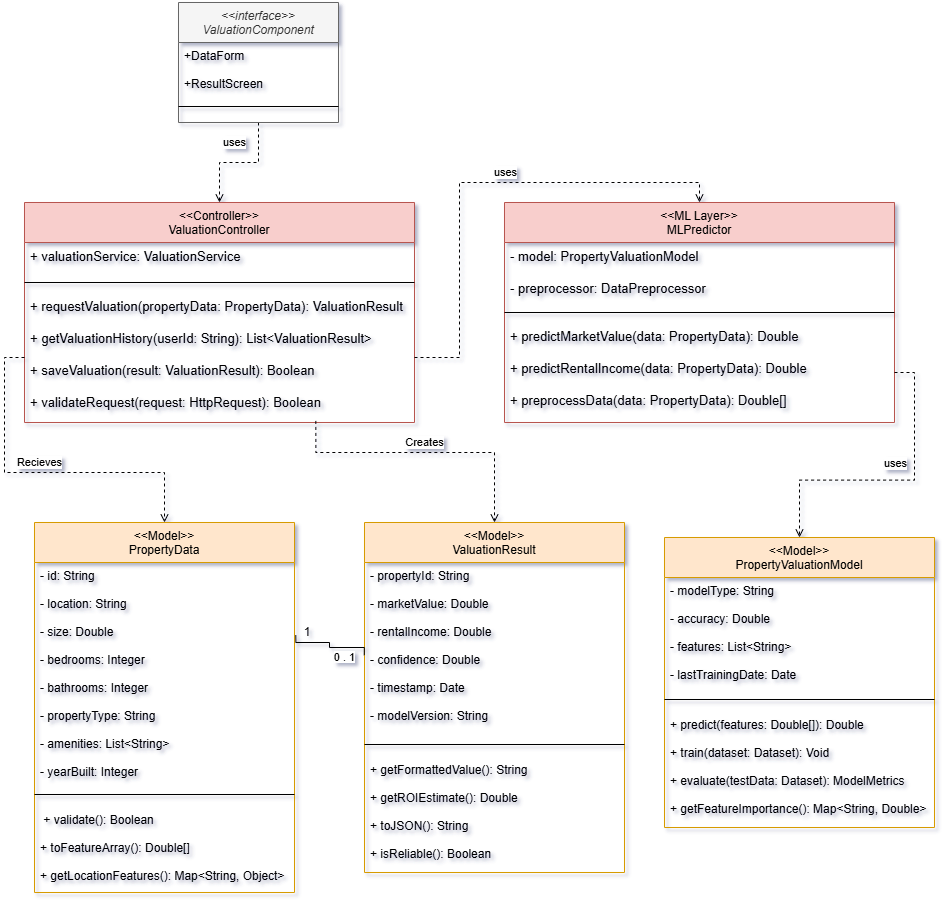
\includegraphics[width=0.9\textwidth]{images/valuation_class_diagram.png}
    \caption{Property Valuation Model Class Diagram}
    \label{fig:valuation-class-diagram}
\end{figure}
\subsection{Model Architecture and Training Process}
\subsubsection{Data Features for Valuation}
The accuracy of the property valuation model heavily relies on the quality and comprehensiveness of the input data. Figure \ref{fig:geo-propriety-data} outlines the key geo-property data features utilized by the model. These features capture essential characteristics of a property and its location, enabling the model to learn complex relationships and predict market values and rental incomes effectively.
\newpage
\begin{figure}[htbp]
    \centering
    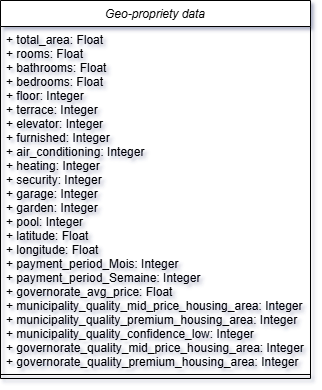
\includegraphics[width=0.4\textwidth]{images/geo-propriety-data.png} % Replace with your actual image path
    \caption{Geo-propriety Data Features for AI Models}
    \label{fig:geo-propriety-data}
\end{figure}

\subsubsection{Model Selection}
To develop an accurate property valuation prediction model, several regression algorithms were evaluated. The following models were selected for training and comparison due to their distinct characteristics and common effectiveness in similar predictive tasks:
\begin{itemize}
    \item \textbf{Linear Regression}: Chosen as a baseline model due to its simplicity and interpretability. It helps in understanding the linear relationships between the features and the target variables (market value and rental income).
    \item \textbf{Random Forest Regressor}: An ensemble learning method that operates by constructing a multitude of decision trees at training time. It is robust to overfitting, handles non-linear relationships well, and often provides high accuracy.
    \item \textbf{Gradient Boosting Regressor}: Another powerful ensemble technique that builds models in a stage-wise fashion. It is known for its high predictive accuracy and ability to optimize for various loss functions, making it suitable for complex regression tasks.
\end{itemize}
These models were trained on the prepared dataset, and their performances were evaluated to select the most suitable one for deployment in the Korpor platform.

\subsubsection{Feature Importance Analysis}
Understanding which features contribute most to the model's predictions is crucial for model interpretability and refinement. After training the selected model, a feature importance analysis was conducted. Figure \ref{fig:feature-importance} displays the top 15 most important features identified by the model. This analysis helps in validating the model's logic.
\newpage

\begin{figure}[htbp]
    \centering
    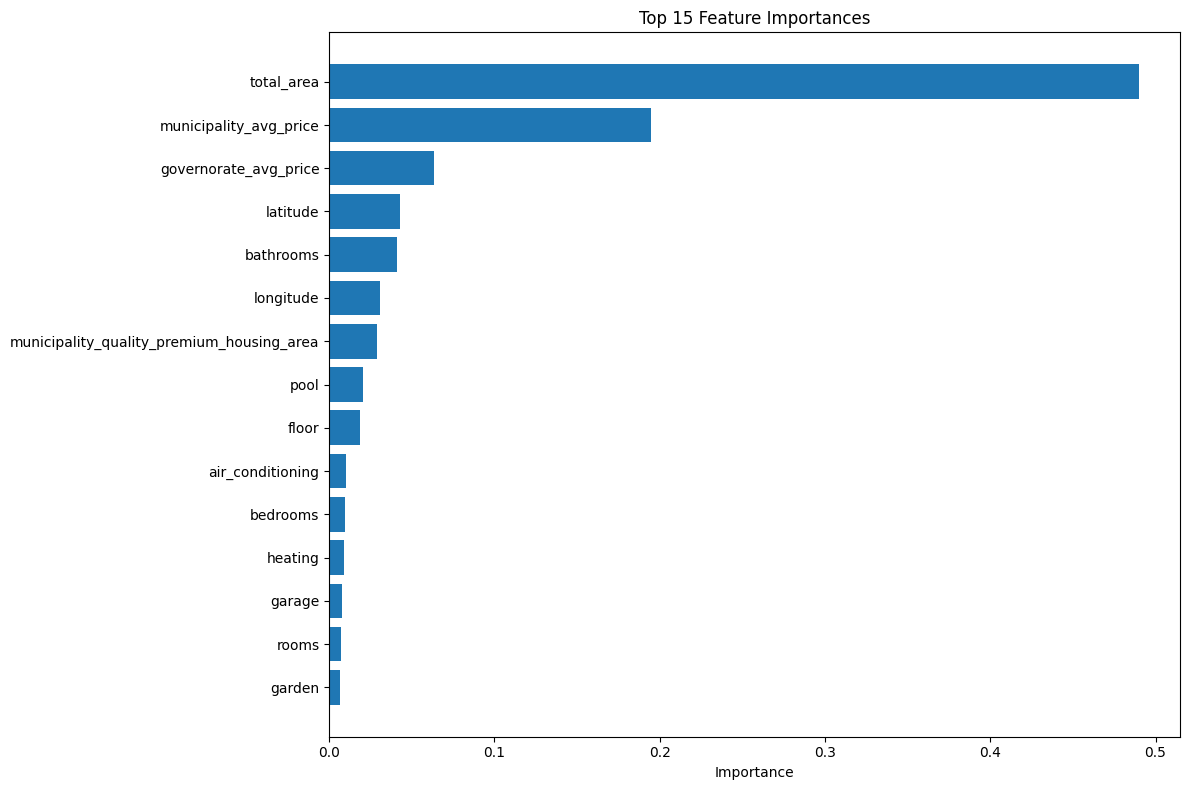
\includegraphics[width=0.8\textwidth]{images/top_15_feature_importance.png} % Assuming image is in 'images' directory
    \caption{Top 15 Feature Importance for Property Valuation Model}
    \label{fig:feature-importance}
\end{figure}

\subsubsection{Model Evaluation and Metrics}
The performance of the trained regression models was rigorously evaluated using standard metrics to ensure reliability and accuracy. Key metrics such as Mean Absolute Error (MAE), Mean Squared Error (MSE), Root Mean Squared Error (RMSE), and R-squared (R²) score were computed on a held-out test dataset. Figure \ref{fig:model-test-metrics} presents a summary of these performance metrics for the chosen valuation model. These results provide a quantitative assessment of the model's ability to generalize to unseen data.


\begin{figure}[htbp]
    \centering
    \begin{minipage}{0.48\textwidth}
        \centering
        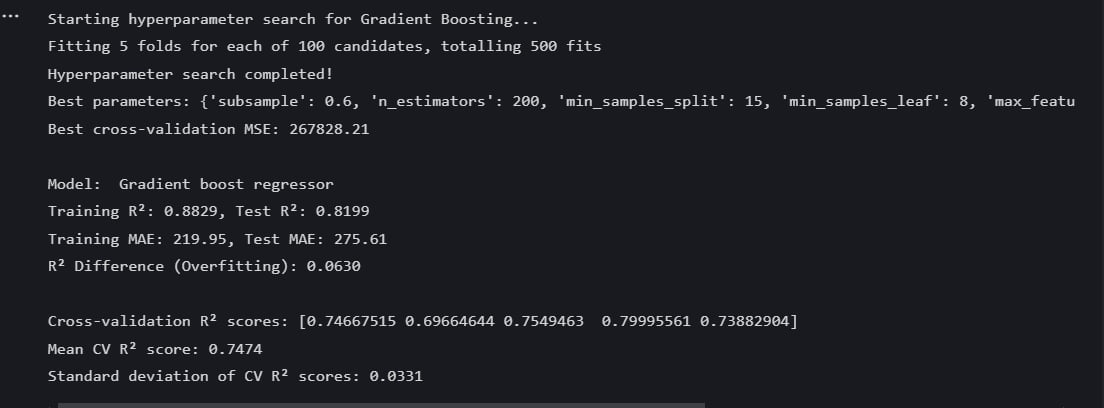
\includegraphics[width=\linewidth]{images/apartmenet location.jpeg}
        \caption*{Apartment Location Prediction}
    \end{minipage}
    \hfill
    \begin{minipage}{0.48\textwidth}
        \centering
        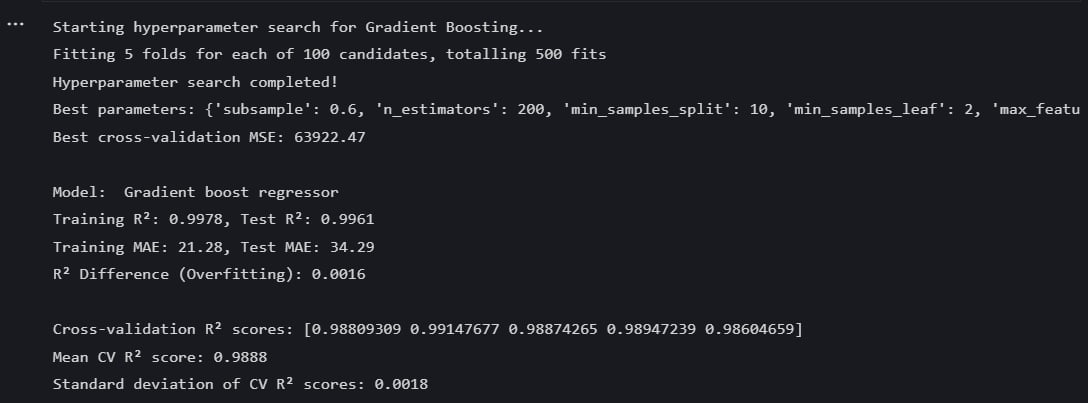
\includegraphics[width=\linewidth]{images/maison location.jpeg}
        \caption*{House Location Prediction}
    \end{minipage}
    
    \vspace{0.5cm}
    
    \begin{minipage}{0.48\textwidth}
        \centering
        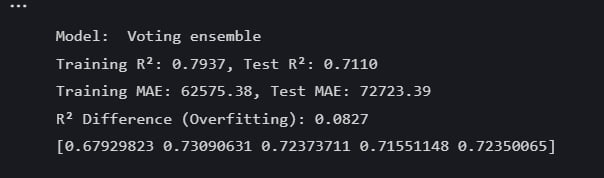
\includegraphics[width=\linewidth]{images/apartmeent vente.jpeg}
        \caption*{Apartment Sale Prediction}
    \end{minipage}
    \hfill
    \begin{minipage}{0.48\textwidth}
        \centering
        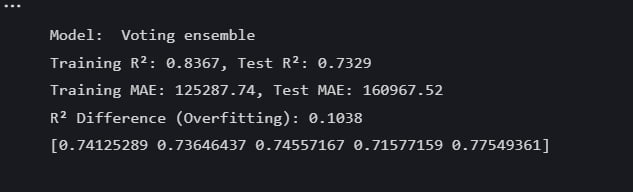
\includegraphics[width=\linewidth]{images/maison vente.jpeg}
        \caption*{House Sale Prediction}
    \end{minipage}
    
    \caption{Prediction Model Test Metrics Summary}
    \label{fig:model-test-metrics}
\end{figure}
\newpage

\subsubsection{Prediction Sequence Flow}
The interaction sequence for the AI property valuation prediction model in Figure \ref{fig:ai-prediction-sequence}.

\begin{figure}[htbp]
    \centering
    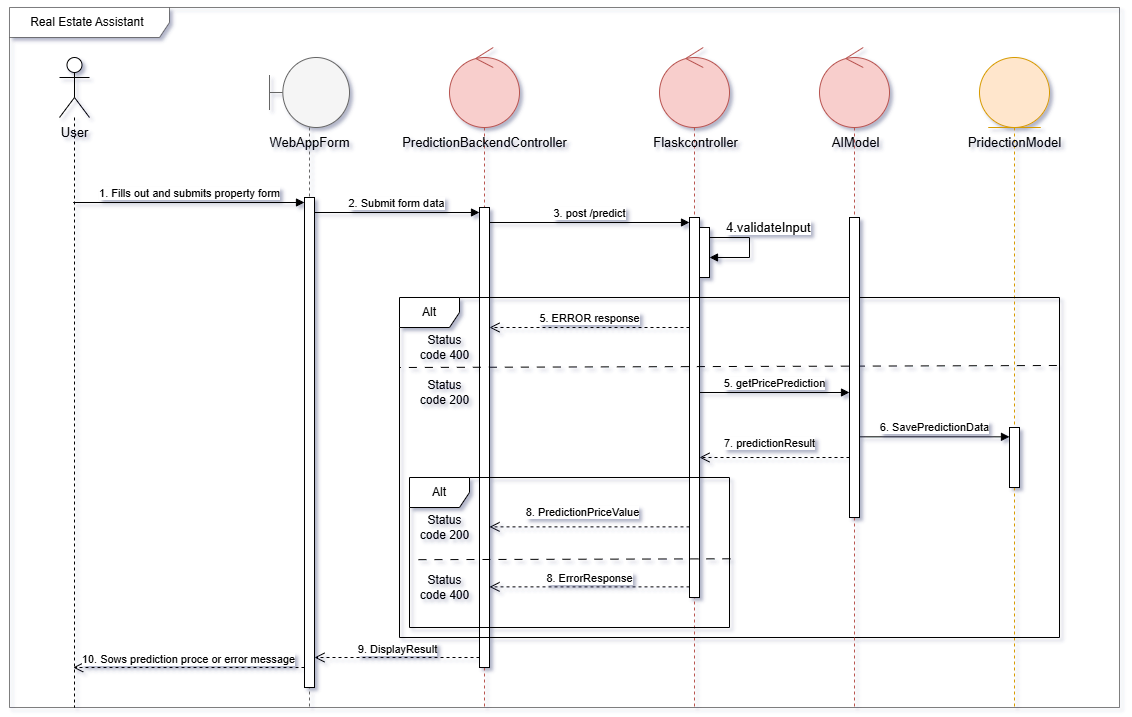
\includegraphics[width=1\textwidth]{images/sequence_AI_prediction_model.png} % Assuming image is in 'images' directory
    \caption{AI Property Valuation Prediction Sequence Diagram}
    \label{fig:ai-prediction-sequence}
\end{figure}


\subsubsection{Prediction User Interface}
Figure \ref{fig:prediction-form} shows the input form, and Figure \ref{fig:prediction-results} displays an example of the prediction results screen.

\begin{figure}[htbp]
        \centering
        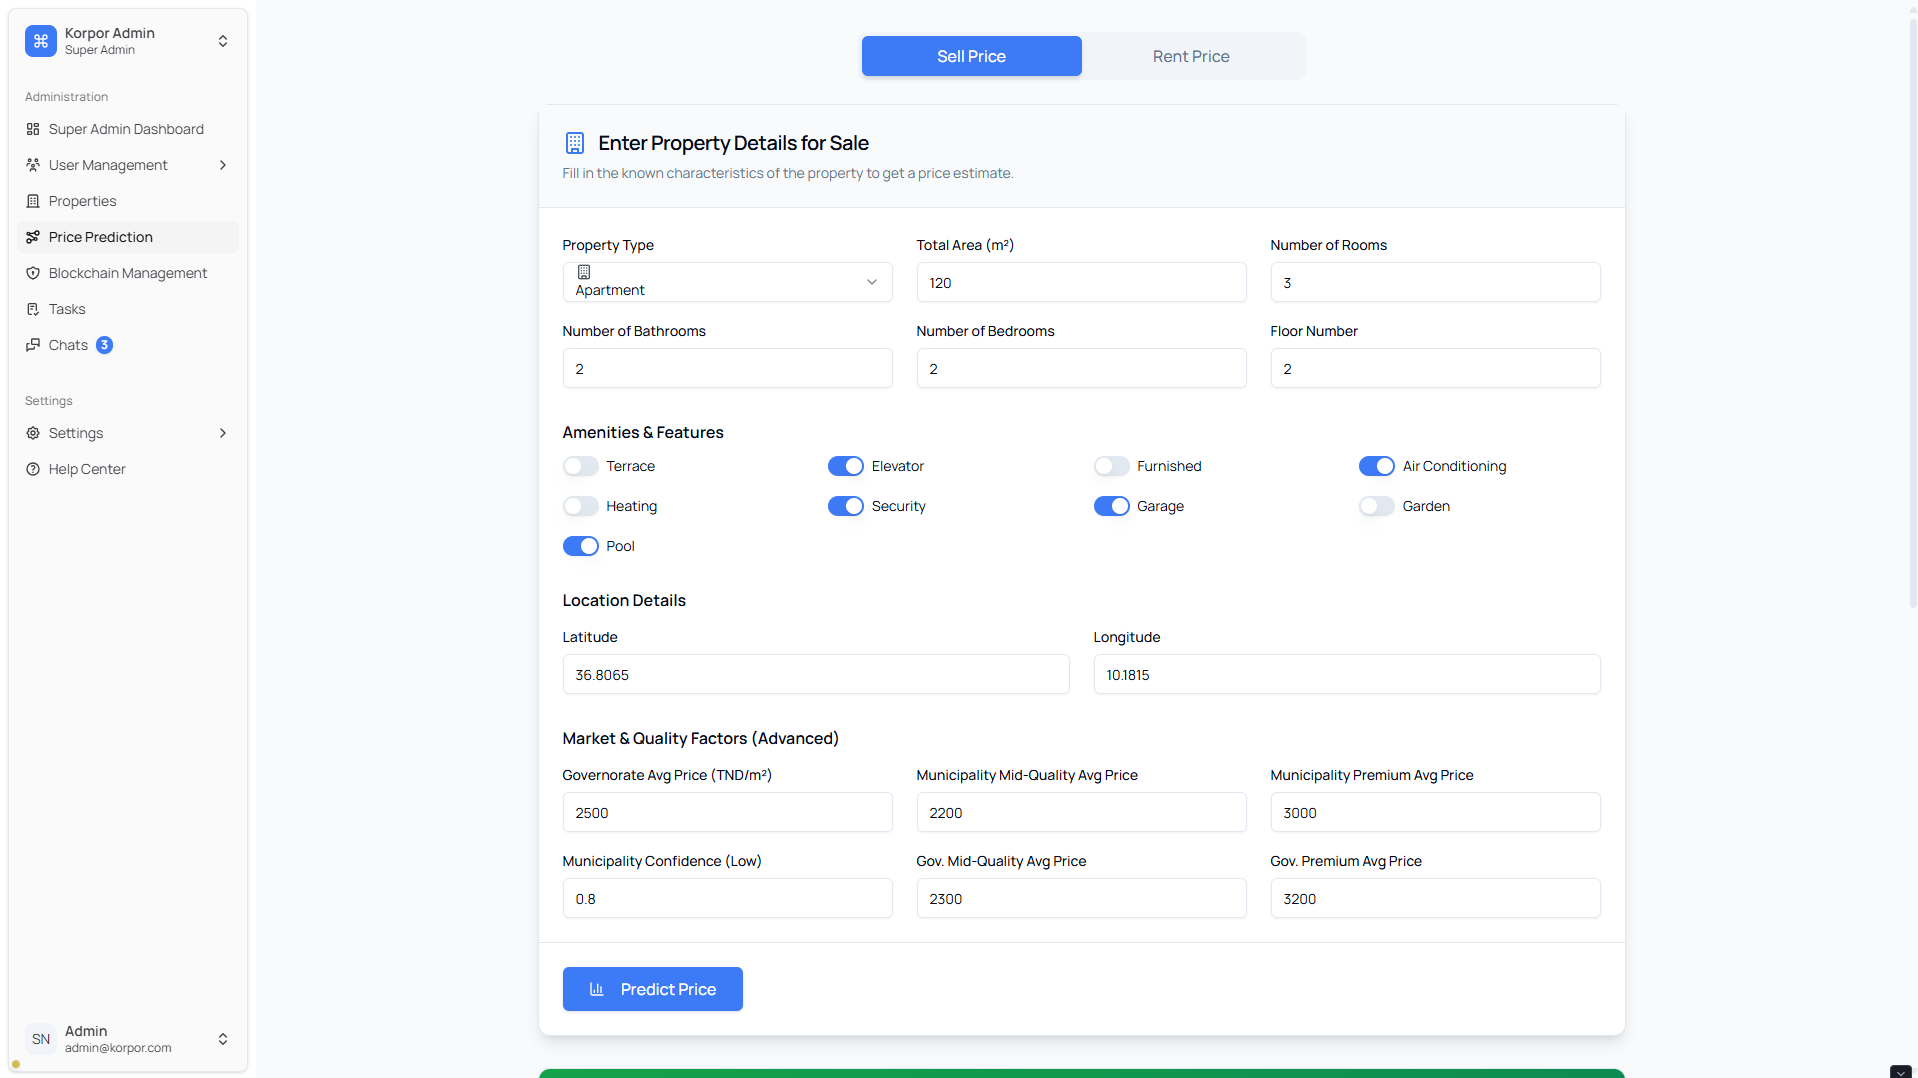
\includegraphics[width=0.7\textwidth]{images/screenshot_form_predition.png}
        \caption{Property Details Input Form for Valuation}
        \label{fig:prediction-form}
\end{figure}

\newpage
\begin{figure}[htbp]
        \centering
        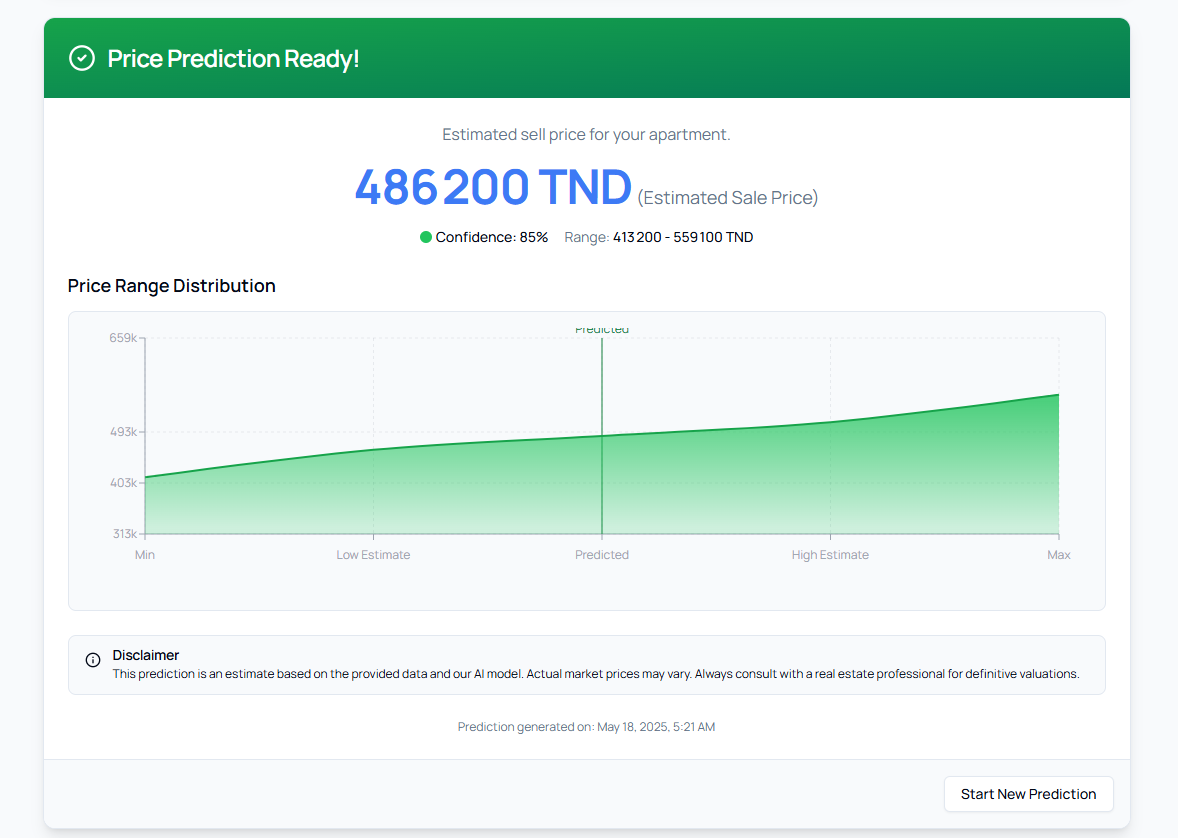
\includegraphics[width=0.7\textwidth]{images/screenshot_predctionscreen.png}
        \caption{Valuation Prediction Results Screen}
        \label{fig:prediction-results}
\end{figure}

\subsubsection{Mobile Investment Insights}
The Korpor mobile application provides investors with direct access to AI-powered property valuations, including future evaluation insights generated by the prediction model. This feature empowers users to make data-driven investment decisions by visualizing potential growth and returns. Figure \ref{fig:mobile-future-evaluation} showcases the mobile interface where these future evaluations are presented to the investor.

\begin{figure}[htbp]
    \centering
    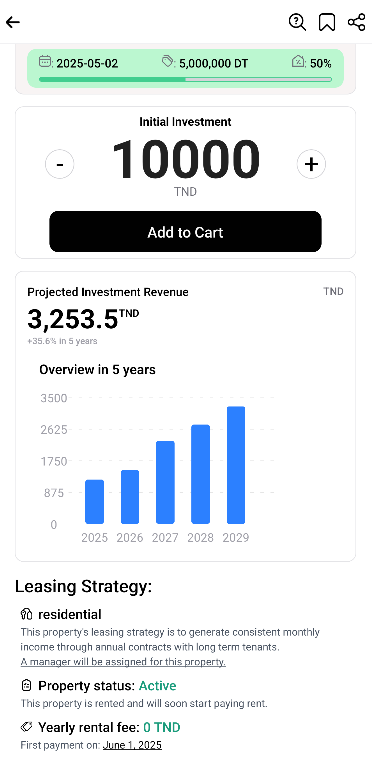
\includegraphics[width=0.3\textwidth]{images/mobile_future_evaluation.png} % Replace with your actual image path
    \caption{Mobile Interface for Future Property Evaluation Insights}
    \label{fig:mobile-future-evaluation}
\end{figure}


\subsubsection{Mobile Interface Testing (Maestro)}
To ensure a seamless and reliable user experience on the mobile platform, the interface for displaying AI-driven property evaluations underwent end-to-end testing using Maestro. The tests covered user flows for accessing predictions and interacting with the displayed data. Figure \ref{fig:maestro-tests-mobile} shows the successful completion of these Maestro tests, validating the robustness of the mobile UI components related to the AI features.

\begin{figure}[htbp]
    \centering
    % \includegraphics[width=0.8\textwidth]{images/maestro_test_mobile_passed.png} % Replace with your actual image path
    \caption{Maestro Test Results for Mobile Prediction Interface}
    \label{fig:maestro-tests-mobile}
\end{figure}

% \begin{table}[htbp]
%     \centering
%     \begin{tabular}{|c|l|l|l|c|}
%         \hline
%         \textbf{Test ID} & \textbf{Scenario} & \textbf{Input} & \textbf{Expected Output} & \textbf{Status} \\
%         \hline
%         VAL-001 & Valid property data & Complete property details & Accurate valuation & \checkmark \\
%         \hline
%         VAL-002 & Incomplete data & Missing property size & Error message & \checkmark \\
%         \hline
%         VAL-003 & Edge case location & Remote area property & Reasonable estimate & \checkmark \\
%         \hline
%         VAL-004 & High-value property & Luxury property details & Premium valuation & \checkmark \\
%         \hline
%         VAL-005 & Model performance & Large dataset & MAE < 10\% & \checkmark \\
%         \hline
%     \end{tabular}
%     \caption{Property Valuation Model Test Scenarios}
%     \label{tab:valuation-test-scenarios}
% \end{table}

\newpage

\section{Sprint 4: Real Estate Assistant (NLP Chatbot)}
\subsection*{Overview}
The Real Estate Assistant is an intelligent NLP-powered chatbot designed to provide investors with instant access to real estate legal information and guidance. This AI assistant helps users understand complex legal concepts, property regulations, and investment procedures through natural language conversations.

\subsection{Requirements Analysis}
\subsubsection{Use Case Diagram}
The Real Estate Assistant serves primarily investors who need legal guidance during their property investment journey. Figure \ref{fig:assistant-use-case} illustrates the main use cases for the AI assistant.
\newpage
\begin{figure}[htbp]
    \centering
    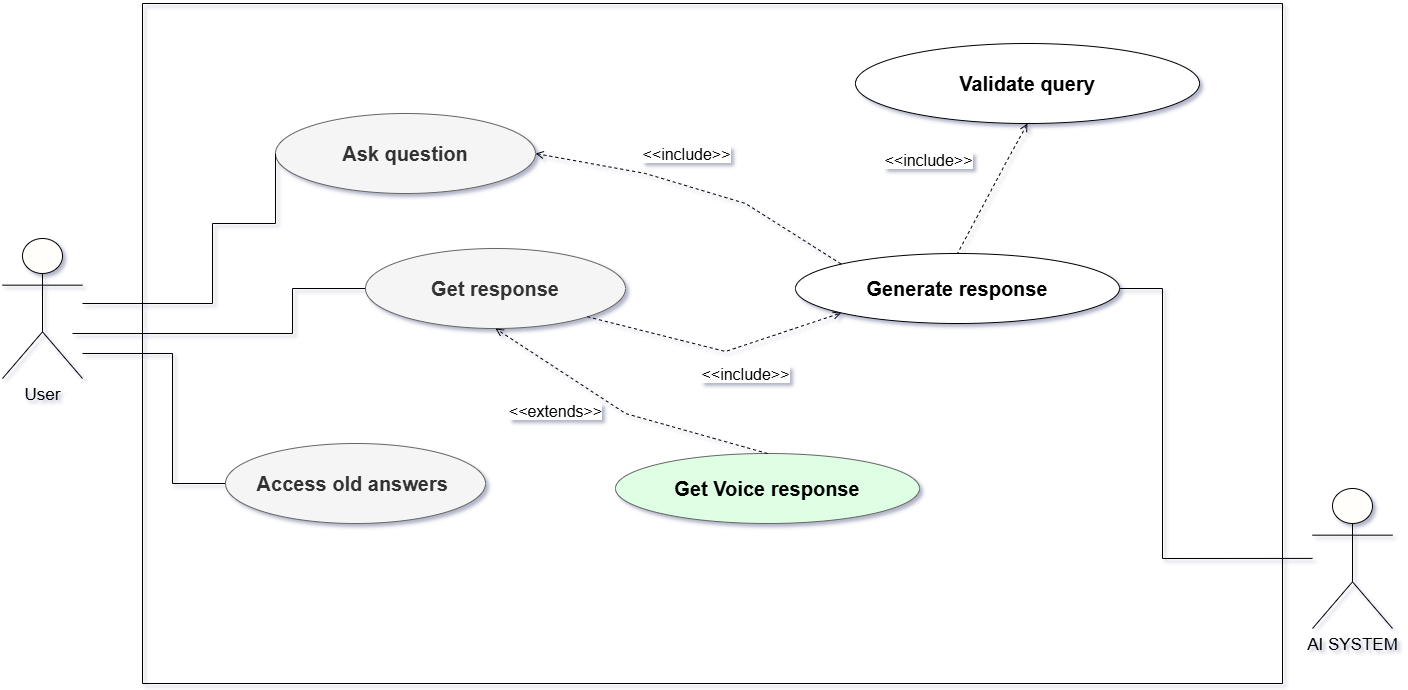
\includegraphics[width=0.9\textwidth]{images/assistant_use_case_diagram.png}
    \caption{Real Estate Assistant Use Case Diagram}
    \label{fig:assistant-use-case}
\end{figure}

\subsubsection{Textual Use Case Descriptions}

\textbf{Use Case: Ask Legal Question}
\begin{itemize}
    \item \textbf{Actor}: Investor
    \item \textbf{Precondition}: User is authenticated and has access to the mobile app
    \item \textbf{Main Flow}: 
    \begin{enumerate}
        \item Investor opens chat interface
        \item Investor types legal question in natural language
        \item System processes question using NLP
        \item System retrieves relevant legal information
        \item System provides comprehensive answer with references
        \item System maintains conversation context for follow-up questions
    \end{enumerate}
    \item \textbf{Alternative Flow}: If question is unclear, system asks for clarification
    \item \textbf{Postcondition}: Conversation is saved for future reference
\end{itemize}

\textbf{Use Case: Provide Legal Guidance}
\begin{itemize}
    \item \textbf{Actor}: System (AI Assistant)
    \item \textbf{Precondition}: User has asked a legal question
    \item \textbf{Main Flow}: 
    \begin{enumerate}
        \item System analyzes question intent and entities
        \item System searches legal knowledge base
        \item System generates contextual response
        \item System provides relevant legal references
        \item System suggests related topics
    \end{enumerate}
    \item \textbf{Postcondition}: User receives accurate legal information
\end{itemize}

\subsection{System Design}
\subsubsection{Class Diagram}
The Real Estate Assistant follows a modular architecture for NLP processing and knowledge management. Figure \ref{fig:assistant-class-diagram} shows the main classes and their relationships.

\begin{figure}[htbp]
    \centering
    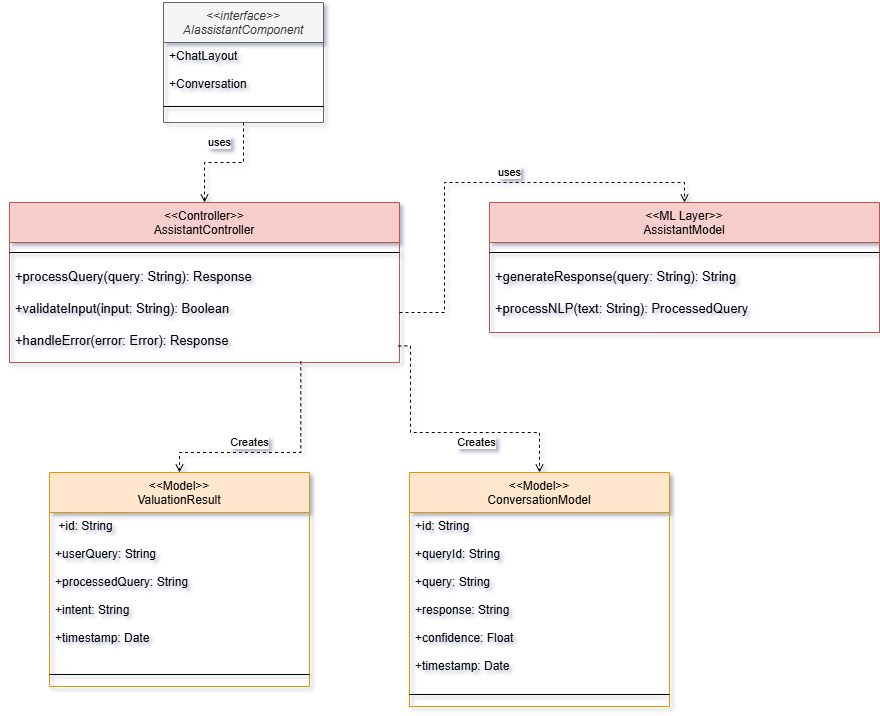
\includegraphics[width=0.8\textwidth]{images/assistant_class_diagram.png}
    \caption{Real Estate Assistant Class Diagram}
    \label{fig:assistant-class-diagram}
\end{figure}

\subsubsection{Sequence Diagram (MVC)}
The interaction flow between the mobile interface, backend services, and NLP processing components is illustrated in Figure \ref{fig:assistant-sequence-mvc}.
\newpage
\begin{figure}[htbp]
    \centering
    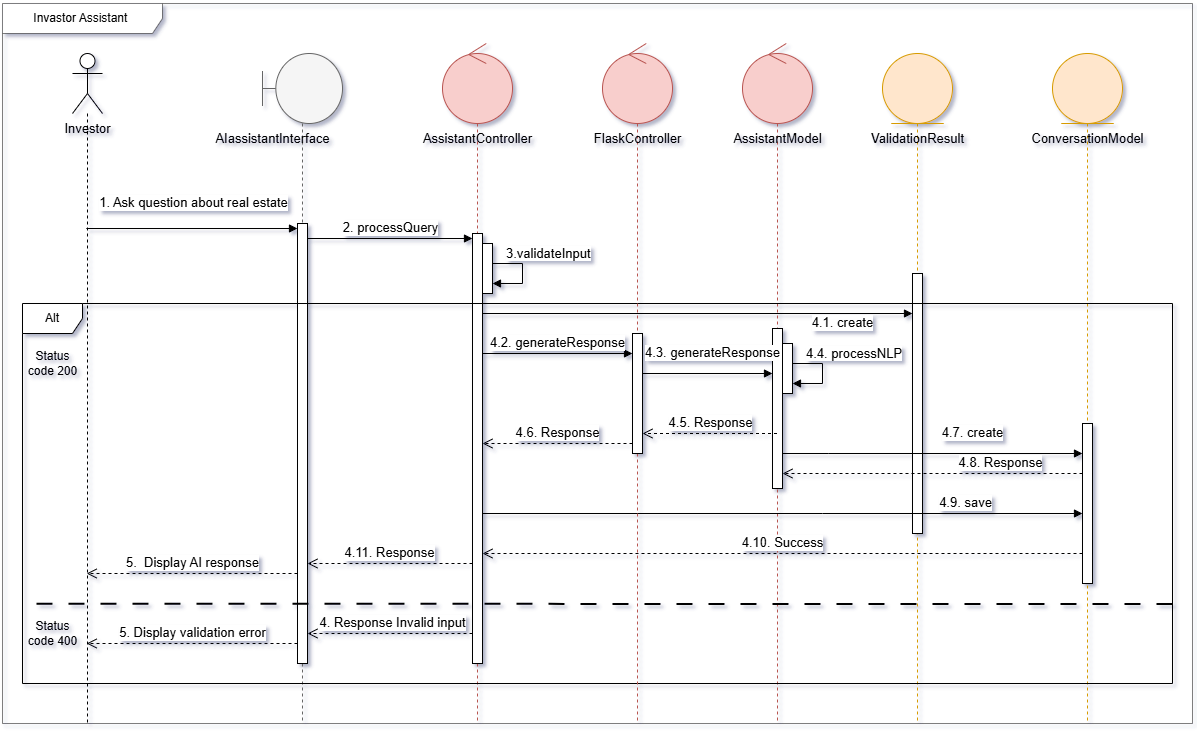
\includegraphics[width=1\textwidth]{images/assistant_sequence_mvc.png}
    \caption{Real Estate Assistant MVC Sequence Diagram}
    \label{fig:assistant-sequence-mvc}
\end{figure}

\subsection{Implementation}
\subsubsection{NLP Model Architecture}
The Real Estate Assistant utilizes advanced natural language processing techniques to understand and respond to user queries. The system employs:

\begin{itemize}
    \item \textbf{Intent Recognition}: Identifies the purpose of user questions (property law, taxes, contracts, etc.)
    \item \textbf{Entity Extraction}: Extracts key information like property types, locations, and legal concepts
    \item \textbf{Context Management}: Maintains conversation history for coherent multi-turn dialogues
    \item \textbf{Response Generation}: Creates natural, informative responses based on legal knowledge base
\end{itemize}

\subsubsection{Legal Knowledge Base}
The assistant's knowledge base contains comprehensive information about:
\begin{itemize}
    \item Tunisian real estate law and regulations
    \item Property investment procedures
    \item Tax implications and calculations
    \item Contract templates and requirements
    \item Common legal issues and solutions
\end{itemize}

\subsubsection{Chat Interface Implementation}
The mobile chat interface provides an intuitive way for investors to interact with the AI assistant. Figure \ref{fig:assistant-mobile-chat} shows the chat interface design.

\begin{figure}[htbp]
    \centering
    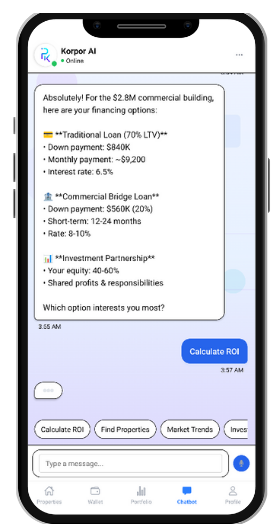
\includegraphics[width=0.3\textwidth]{images/assistant_mobile_chat.png}
    \caption{Mobile Chat Interface for Real Estate Assistant}
    \label{fig:assistant-mobile-chat}
\end{figure}


\subsection{Testing and Validation}
\subsubsection{Test Scenarios}
The Real Estate Assistant underwent extensive testing to ensure accurate responses and reliable performance. Table \ref{tab:assistant-test-scenarios} presents the key test scenarios.

\begin{table}[htbp]
    \centering
    \begin{tabular}{|c|l|l|l|c|}
        \hline
        \textbf{Scenario} & \textbf{Input} & \textbf{Expected Output} & \textbf{Status} \\
        \hline
         Property tax query & "What are property taxes?" & Detailed tax information & \checkmark \\
        \hline
        Contract question & "What's in a rental contract?" & Contract requirements & \checkmark \\
        \hline
         Investment procedure & "How to buy property?" & Step-by-step guide & \checkmark \\
        \hline
         Legal compliance & "Foreign investment rules?" & Regulatory information & \checkmark \\
        \hline
         Context follow-up & Multi-turn conversation & Coherent responses & \checkmark \\
        \hline
         Unclear question & Ambiguous query & Clarification request & \checkmark \\
        \hline
    \end{tabular}
    \caption{Real Estate Assistant Test Scenarios}
    \label{tab:assistant-test-scenarios}
\end{table}

\newpage

\section{Role-Based Backoffice Agent}
\subsection*{Overview}
The Role-Based Backoffice Agent is an intelligent AI system designed to assist different user roles (Super Admin, Admin, Real Estate Agent) with automated task management, workflow optimization, and decision support. This AI agent adapts its behavior and recommendations based on the specific role and responsibilities of the authenticated user.

\subsection{Requirements Analysis}
\subsubsection{Use Case Diagram}
The Role-Based Backoffice Agent serves multiple user types with role-specific functionalities and automated assistance. Figure \ref{fig:backoffice-use-case} illustrates the main use cases for each role.

\begin{figure}[htbp]
    \centering
    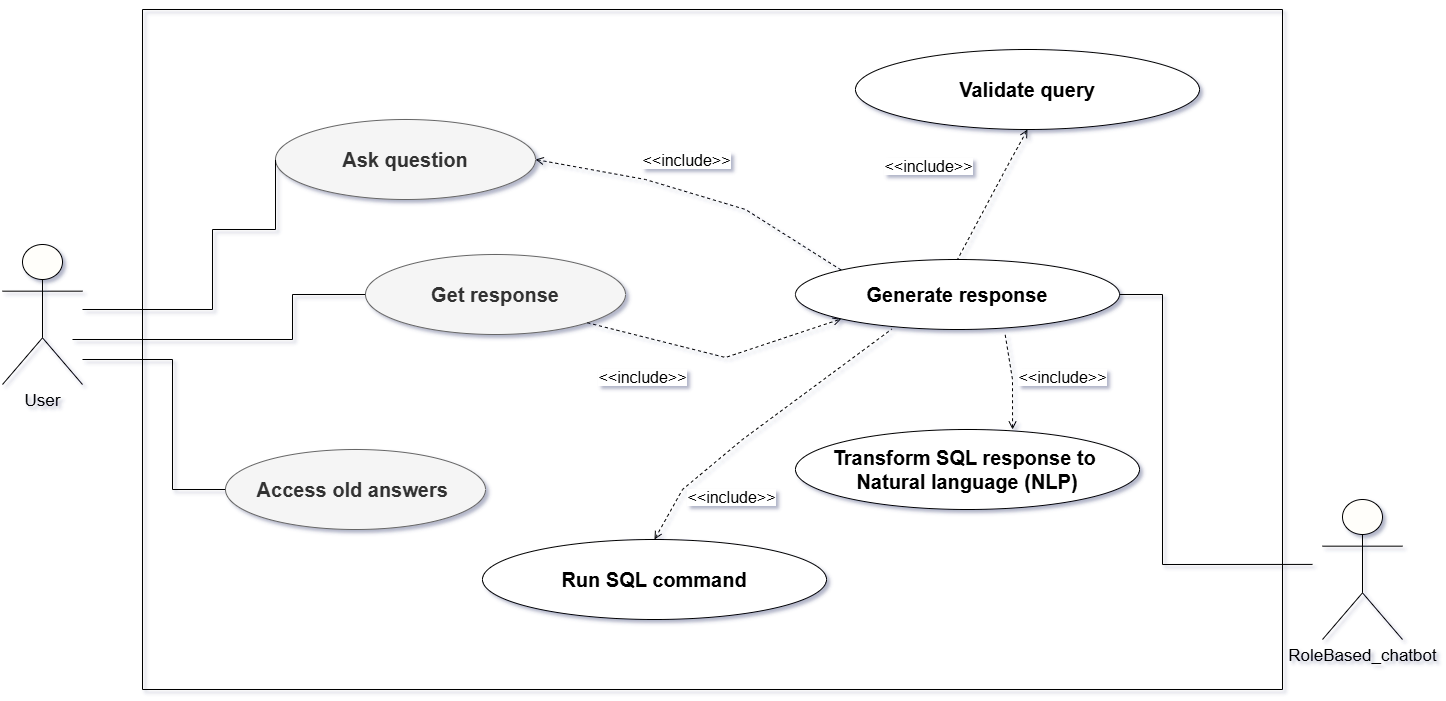
\includegraphics[width=1\textwidth]{images/backoffice_use_case_diagram.png}
    \caption{Role-Based Backoffice Agent Use Case Diagram}
    \label{fig:backoffice-use-case}
\end{figure}

\subsubsection{Textual Use Case Descriptions}

\textbf{Use Case: Automate Task Management}
\begin{itemize}
    \item \textbf{Actor}: User (representing Super Admin, Admin, Real Estate Agent)
    \item \textbf{Precondition}: User is authenticated with specific role permissions
    \item \textbf{Main Flow}: 
    \begin{enumerate}
        \item User accesses backoffice dashboard
        \item System identifies user role and permissions
        \item AI agent analyzes pending tasks and priorities
        \item System suggests automated actions based on role
        \item User approves or modifies suggested actions
        \item System executes approved automated tasks
    \end{enumerate}
    \item \textbf{Alternative Flow}: If automation requires approval, system queues for manual review
    \item \textbf{Postcondition}: Tasks are efficiently managed with minimal manual intervention
\end{itemize}

\textbf{Use Case: Provide Role-Specific Insights}
\begin{itemize}
    \item \textbf{Actor}: AI Agent
    \item \textbf{Precondition}: User has accessed dashboard with specific role
    \item \textbf{Main Flow}: 
    \begin{enumerate}
        \item System analyzes user role and current context
        \item AI generates role-specific insights 
        \item AI suggests optimization opportunities
        \item System provides actionable recommendations
    \end{enumerate}
    \item \textbf{Postcondition}: User receives personalized insights for their role
\end{itemize}

\subsection{System Design}
\subsubsection{Class Diagram}
The Role-Based Backoffice Agent follows a role-based architecture with specialized services for each user type. Figure \ref{fig:backoffice-class-diagram} shows the main classes and their relationships.
\newpage
\begin{figure}[htbp]
    \centering
    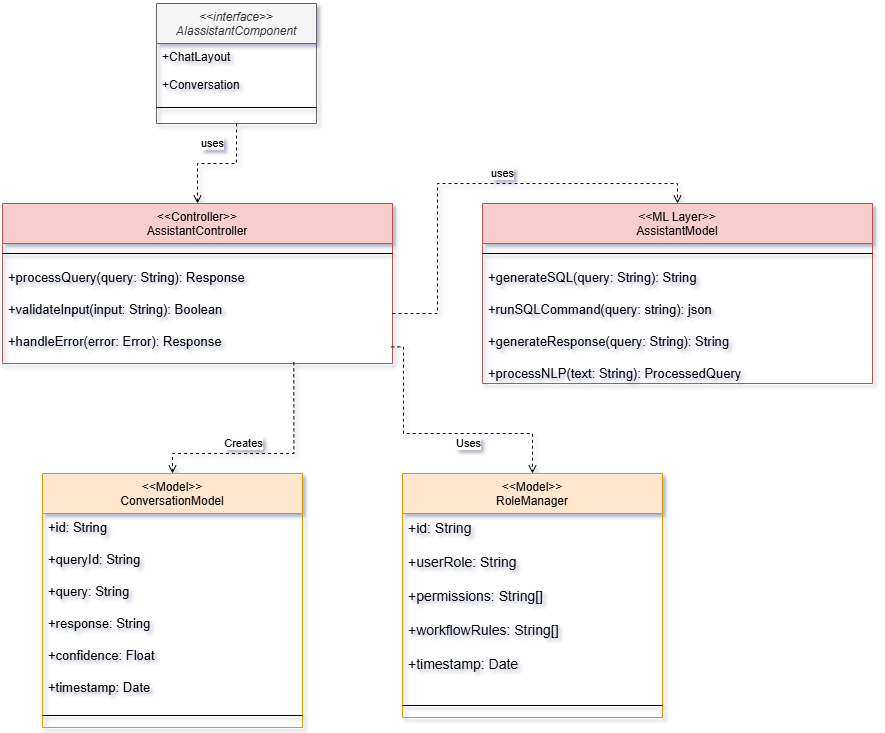
\includegraphics[width=1\textwidth]{images/backoffice_class_diagram.png}
    \caption{Role-Based Backoffice Agent Class Diagram}
    \label{fig:backoffice-class-diagram}
\end{figure}

\subsubsection{Sequence Diagram (MVC)}
The interaction flow between the web interface, role management services, and AI processing components is illustrated in Figure \ref{fig:backoffice-sequence-mvc}.
\newpage
\begin{figure}[htbp]
    \centering
    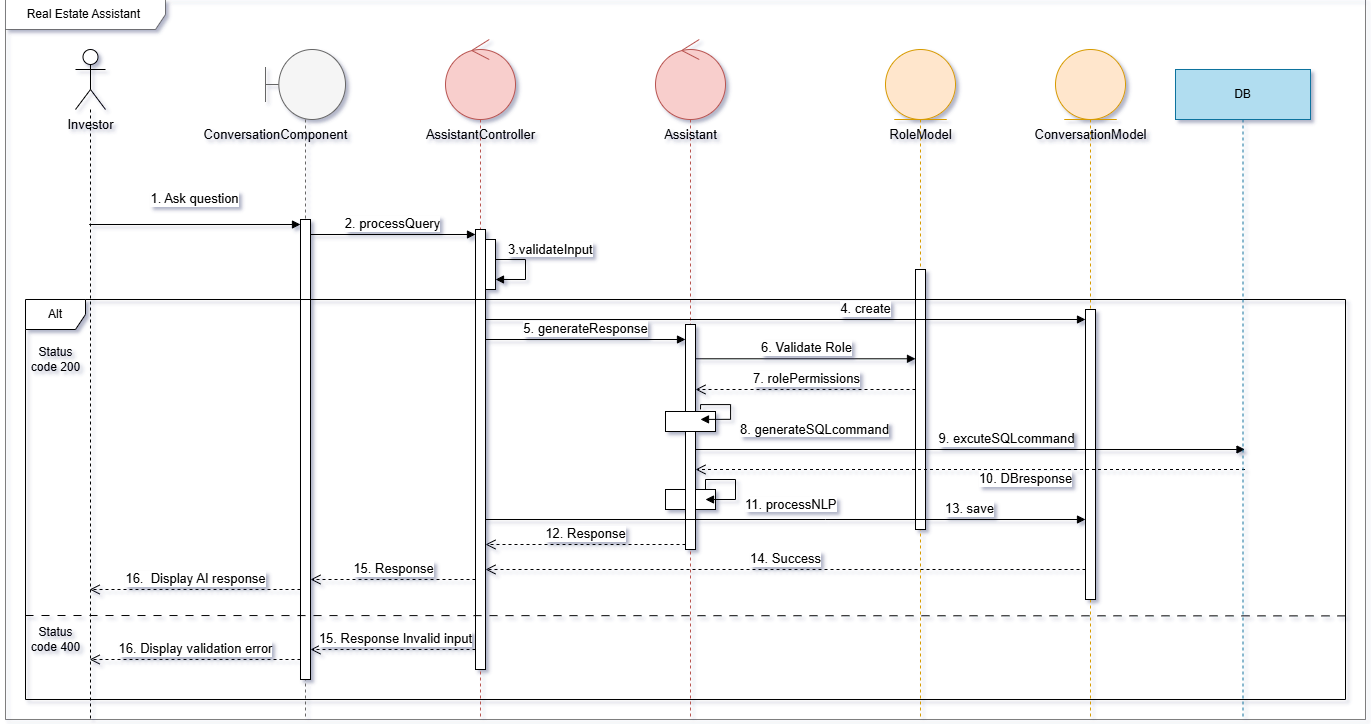
\includegraphics[width=1\textwidth]{images/backoffice_sequence_mvc.png}
    \caption{Role-Based Backoffice Agent MVC Sequence Diagram}
    \label{fig:backoffice-sequence-mvc}
\end{figure}

\subsection{Implementation}
\subsubsection{Role-Based AI Logic}
The Backoffice Agent utilizes sophisticated role-based AI algorithms to provide personalized assistance:

\begin{itemize}
    \item \textbf{Super Admin Features}: System monitoring, user management, platform analytics, security oversight
    \item \textbf{Admin Features}: Property management, user support, content moderation, performance tracking
    \item \textbf{Real Estate Agent Features}: Client management, property listings, sales tracking, commission calculations
\end{itemize}

\subsubsection{Automated Workflow Management}
The system automates routine tasks based on role permissions:
\begin{itemize}
    \item Property approval workflows for admins
    \item User verification processes for super admins
    \item Client follow-up reminders for agents
    \item Performance report generation for all roles
\end{itemize}

\newpage
\subsubsection{Dashboard Implementation}
Each role receives a customized dashboard with relevant tools and insights. Figure \ref{fig:backoffice-dashboard} shows the role-specific dashboard implementations.

\begin{figure}[htbp]
    \centering
    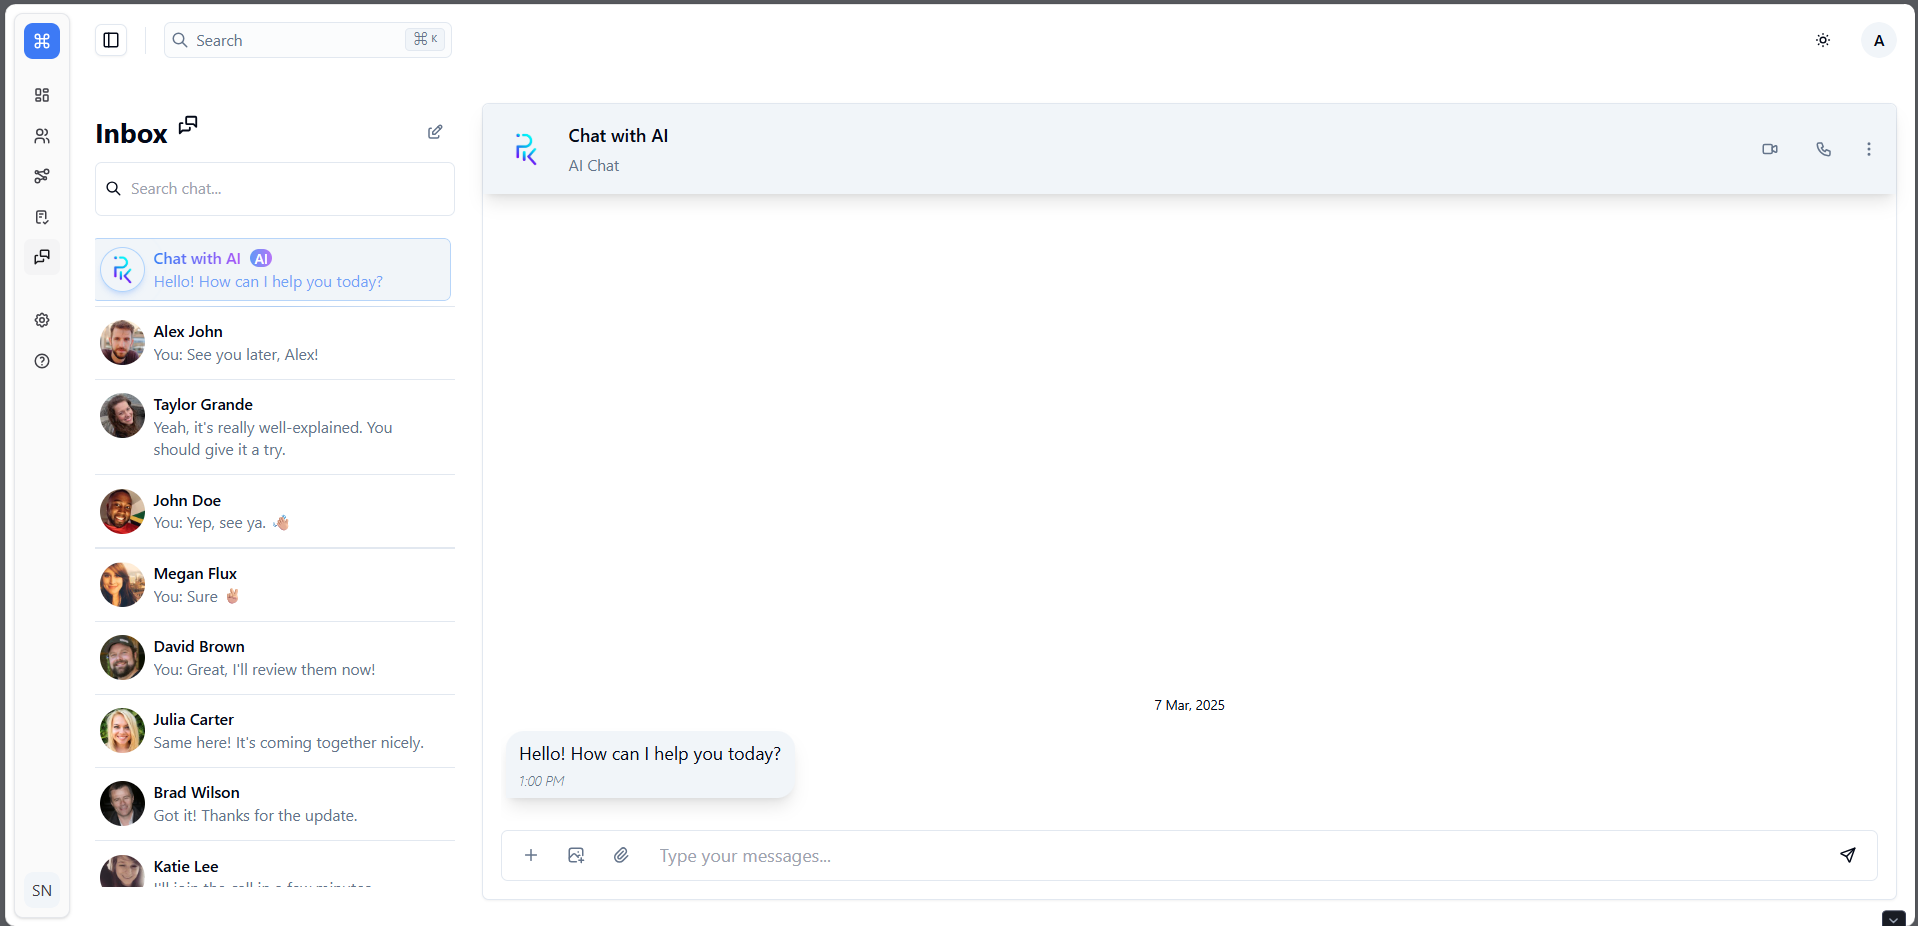
\includegraphics[width=1\textwidth]{images/assistant_web_interface.png}
    \caption{Web Interface for Real Estate Assistant}
    \label{fig:assistant-web-interface}
\end{figure}


\subsection{Testing and Validation}
\subsubsection{Test Scenarios}
The Role-Based Backoffice Agent underwent comprehensive testing across all user roles. Table \ref{tab:backoffice-test-scenarios} presents the key test scenarios.

\begin{table}[htbp]
    \centering
    \begin{tabular}{|c|l|l|l|c|}
        \hline
        \textbf{Scenario} & \textbf{User Role} & \textbf{Expected Output} & \textbf{Status} \\
        \hline
        Role identification & Super Admin & Admin dashboard access & \checkmark \\
        \hline
        Task automation & Admin & Property approval workflow & \checkmark \\
        \hline
        Performance insights & Real Estate Agent & Sales analytics & \checkmark \\
        \hline
        Permission validation & Admin & Restricted super admin features & \checkmark \\
        \hline
        AI recommendations & All roles & Role-specific suggestions & \checkmark \\
        \hline
        Workflow management & Super Admin & System optimization tips & \checkmark \\
        \hline
    \end{tabular}
    \caption{Role-Based Backoffice Agent Test Scenarios}
    \label{tab:backoffice-test-scenarios}
\end{table}
\newpage
\section{Sprint 5: Investor-Focused Recommendation System}
\subsection*{Overview}
The Investor-Focused Recommendation System is an advanced AI model that analyzes investor behavior, preferences, and market conditions to provide personalized property investment recommendations. This system leverages machine learning algorithms to match investors with optimal investment opportunities based on their risk profile, budget, and investment goals.

\begin{figure}[htbp]
    \centering
    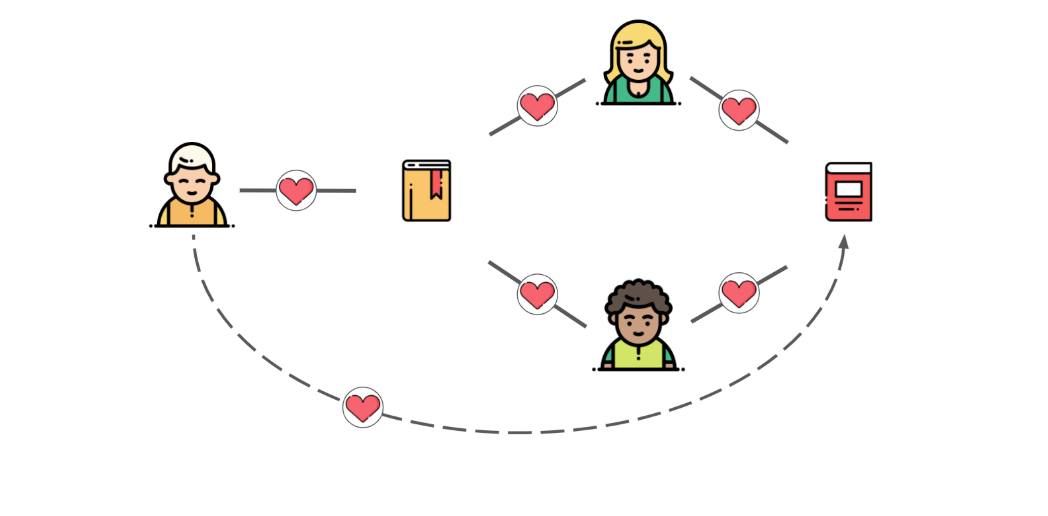
\includegraphics[width=0.7\textwidth]{images/collaborative_filtring.png}
    \caption{Collaborative Filtering Recommendation System Overview}
    \label{fig:collaborative-filtering-overview}
\end{figure}

\subsection{Requirements Analysis}
\subsubsection{Use Case Diagram}
The Recommendation System serves investors by analyzing their profiles and suggesting suitable investment opportunities. Figure \ref{fig:recommendation-use-case} illustrates the main use cases for the recommendation engine.

\begin{figure}[htbp]
    \centering
    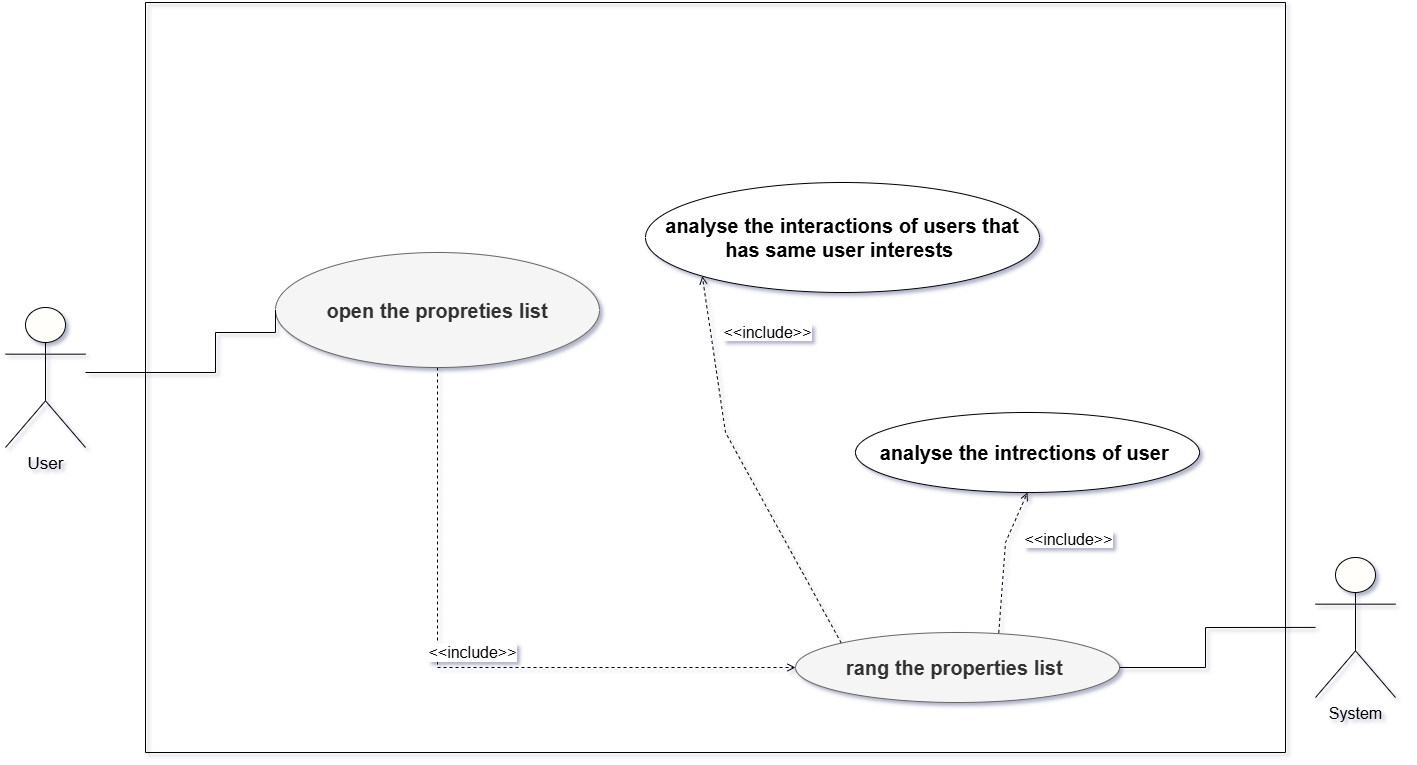
\includegraphics[width=0.7\textwidth]{images/recommendation_use_case_diagram.png}
    \caption{Investor-Focused Recommendation System Use Case Diagram}
    \label{fig:recommendation-use-case}
\end{figure}

\subsubsection{Textual Use Case Descriptions}

\textbf{Use Case: Generate Investment Recommendations}
\begin{itemize}
    \item \textbf{Actor}: User (Investor)
    \item \textbf{Precondition}: Investor has completed profile setup and preferences
    \item \textbf{Main Flow}: 
    \begin{enumerate}
        \item Investor accesses recommendations section
        \item System analyzes investor profile and preferences
        \item AI processes available investment opportunities
        \item System matches properties with investor criteria
        \item AI ranks recommendations by compatibility score
        \item System presents personalized investment suggestions
    \end{enumerate}
    \item \textbf{Alternative Flow}: If no suitable matches, system suggests expanding criteria
    \item \textbf{Postcondition}: Investor receives tailored investment recommendations
\end{itemize}

\textbf{Use Case: Update Investment Preferences}
\begin{itemize}
    \item \textbf{Actor}: Investor
    \item \textbf{Precondition}: Investor is authenticated and has existing profile
    \item \textbf{Main Flow}: 
    \begin{enumerate}
        \item Investor accesses preference settings
        \item User modifies risk tolerance, budget, or location preferences
        \item System validates and saves updated preferences
        \item AI recalculates recommendation algorithms
        \item System generates new recommendations based on updated profile
    \end{enumerate}
    \item \textbf{Postcondition}: Recommendations are updated to reflect new preferences
\end{itemize}

\subsection{System Design}
\subsubsection{Class Diagram}
The Recommendation System uses collaborative filtering and content-based algorithms for personalized suggestions. Figure \ref{fig:recommendation-class-diagram} shows the main classes and their relationships.

\begin{figure}[htbp]
    \centering
    % 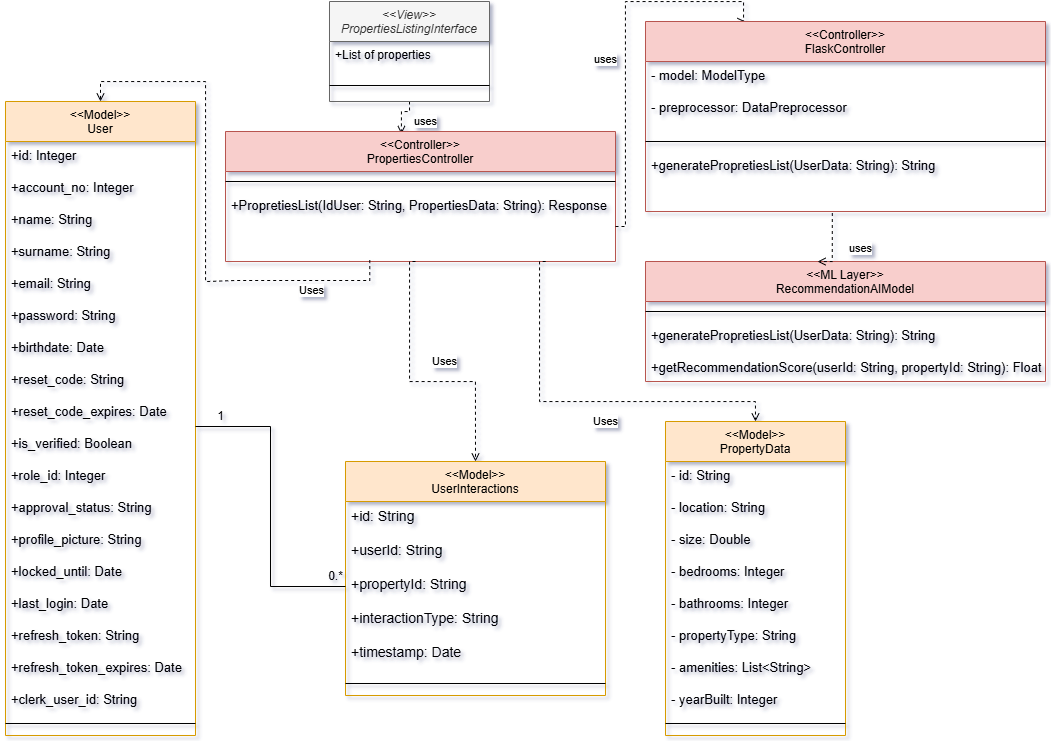
\includegraphics[width=0.8\textwidth]{images/recommendation_class_diagram.png}
    \caption{Investor-Focused Recommendation System Class Diagram}
    \label{fig:recommendation-class-diagram}
\end{figure}

\subsubsection{Sequence Diagram (MVC)}
The interaction flow between the mobile interface, recommendation engine, and machine learning components is illustrated in Figure \ref{fig:recommendation-sequence-mvc}.

\begin{figure}[htbp]
    \centering
    % 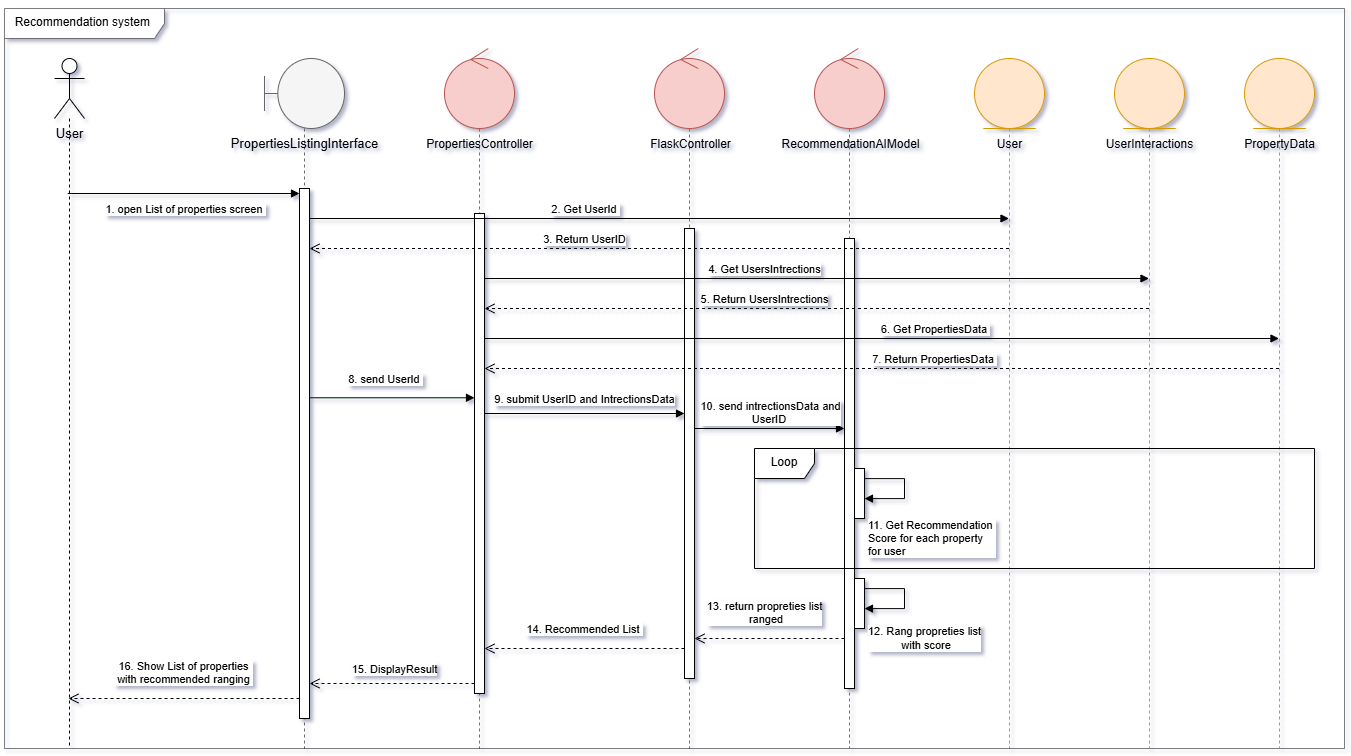
\includegraphics[width=1\textwidth]{images/recommendation_sequence_mvc.png}
    \caption{Recommendation System MVC Sequence Diagram}
    \label{fig:recommendation-sequence-mvc}
\end{figure}

\subsection{Implementation}
\subsubsection{Machine Learning Algorithms}
The Recommendation System employs multiple ML techniques for optimal suggestions:

\begin{itemize}
    \item \textbf{Collaborative Filtering}: Analyzes similar investor behaviors and preferences
    \item \textbf{Content-Based Filtering}: Matches properties based on investor criteria
    \item \textbf{Hybrid Approach}: Combines multiple algorithms for enhanced accuracy
    \item \textbf{Deep Learning}: Neural networks for complex pattern recognition
\end{itemize}

\subsubsection{Investor Profiling}
The system creates comprehensive investor profiles including:
\begin{itemize}
    \item Risk tolerance assessment
    \item Investment budget and timeline
    \item Geographic preferences
    \item Property type preferences
    \item Previous investment history
    \item Market behavior analysis
\end{itemize}

\subsubsection{Mobile Recommendations Interface}
The mobile app provides an intuitive interface for viewing personalized recommendations. Figure \ref{fig:recommendation-mobile} shows the mobile recommendation implementation.

\begin{figure}[htbp]
    \centering
    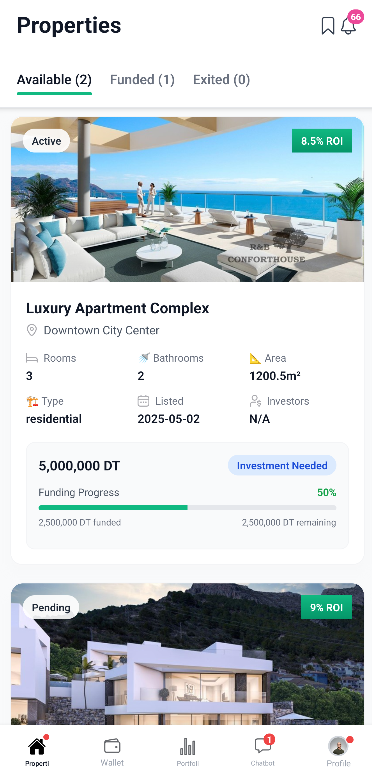
\includegraphics[width=0.3\textwidth]{images/recommendation_mobile.png}
    \caption{Mobile Interface for Investment Recommendations}
    \label{fig:recommendation-mobile}
\end{figure}

\subsubsection{Recommendation Algorithm Visualization}
The system provides transparency in recommendation logic through visual explanations. Figure \ref{fig:recommendation-algorithm} demonstrates how recommendations are generated and explained to users.

\begin{figure}[htbp]
    \centering
    % \includegraphics[width=0.8\textwidth]{images/recommendation_algorithm.png}
    \caption{Recommendation Algorithm Visualization}
    \label{fig:recommendation-algorithm}
\end{figure}

\subsubsection{Personalized Dashboard}
Investors receive a personalized dashboard with recommendations and portfolio insights. Figure \ref{fig:recommendation-dashboard} shows the recommendation dashboard design.


\subsection{Testing and Validation}
\subsubsection{Test Scenarios}
The Recommendation System underwent extensive testing to ensure accuracy and relevance. Table \ref{tab:recommendation-test-scenarios} presents the key test scenarios.

\begin{table}[htbp]
    \centering
    \begin{tabular}{|c|l|l|l|c|}
        \hline
        \textbf{Scenario} & \textbf{Input} & \textbf{Expected Output} & \textbf{Status} \\
        \hline
        New investor profile & Basic preferences & Relevant recommendations & \checkmark \\
        \hline
        Preference update & Changed risk tolerance & Updated suggestions & \checkmark \\
        \hline
        Budget constraint & Limited budget & Affordable options & \checkmark \\
        \hline
         Location preference & Specific city & Local properties & \checkmark \\
        \hline
        Algorithm accuracy & Historical data & High precision score & \checkmark \\
        \hline
        Performance optimization & Large dataset & Fast response time & \checkmark \\
        \hline
    \end{tabular}
    \caption{Recommendation System Test Scenarios}
    \label{tab:recommendation-test-scenarios}
\end{table}


\subsubsection{Mobile App Testing (Maestro)}
The mobile recommendation interface underwent thorough testing using Maestro to ensure optimal user experience. Figure \ref{fig:maestro-recommendation} shows the successful test execution.

\begin{figure}[htbp]
    \centering
    % \includegraphics[width=0.8\textwidth]{images/maestro_recommendation_tests.png}
    \caption{Maestro Test Results for Recommendation System}
    \label{fig:maestro-recommendation}
\end{figure}





